\documentclass[a4paper,11pt]{article}

\usepackage[a4paper,margin=2cm]{geometry}
\usepackage[T1]{fontenc}
\usepackage[utf8]{inputenc}
\usepackage[ngerman,english]{babel}
\usepackage{lmodern}
\usepackage{microtype}
\usepackage{xcolor}
\usepackage{parskip}
\usepackage{enumitem}
\usepackage[most]{tcolorbox}
\usepackage{titlesec}
\usepackage[hidelinks]{hyperref}

\definecolor{HeaderBlueDark}{RGB}{70,110,170}
\definecolor{RowBlueLight}{RGB}{235,243,255}
\definecolor{RowBlueDark}{RGB}{220,233,250}
\definecolor{SoftGray}{RGB}{90,90,90}

\setlength{\parindent}{0pt}
\setlist[itemize]{leftmargin=1.4em,itemsep=0.55em,topsep=0.4em}
\linespread{1.06}

\titleformat{\section}[block]
{\Large\bfseries\color{HeaderBlueDark}}
{}{0pt}{}
\titlespacing{\section}{0pt}{1.3em}{0.8em}

\newtcolorbox{taskbox}{enhanced,breakable,colback=white,colframe=HeaderBlueDark,boxrule=0.6pt,arc=1.5mm,left=2mm,right=2mm,top=1.5mm,bottom=1.5mm}

\newtcolorbox{infobox}{enhanced,breakable,colback=RowBlueLight,colframe=RowBlueDark,boxrule=0.4pt,arc=1.5mm,left=2mm,right=2mm,top=1.5mm,bottom=1.5mm}

\newcommand{\GermanText}[1]{\textbf{Deutsch: }#1\par}
\newcommand{\EnglishText}[1]{{\small\color{SoftGray}\textbf{English: }#1\par}}

\title{Sollten Menschen häufiger mit öffentlichen Verkehrsmitteln fahren?\\[0.35em]
\large \textnormal{Should people use public transportation more often?}}
\date{}

\begin{document}

   \maketitle

   \section{Thema \textnormal{(Topic)}}

      \begin{taskbox}
         \GermanText{In vielen Städten gibt es immer mehr Autos. Dadurch entstehen Staus, Lärm und Luftverschmutzung. Gleichzeitig investieren viele Städte in Busse, Straßenbahnen und U-Bahnen.}
         \EnglishText{In many cities there are more and more cars. This causes traffic jams, noise, and air pollution. At the same time, many cities are investing in buses, trams, and underground trains.}
      \end{taskbox}

   \section{Aufgabe \textnormal{(Task)}}

      \begin{taskbox}
         \GermanText{Schreiben Sie einen Text über das Thema: \textbf{Sollten Menschen häufiger mit öffentlichen Verkehrsmitteln fahren?}}
         \EnglishText{Write a text about the topic: \textbf{Should people use public transportation more often?}}

         \vspace{0.5em}

         \GermanText{Gehen Sie dabei auf die folgenden Punkte ein:}
         \EnglishText{Address the following points:}

         \begin{itemize}
            \item \textbf{Welche Vorteile haben öffentliche Verkehrsmittel?}\\
            {\small\color{SoftGray}What advantages does public transportation have?}

            \item \textbf{Welche Nachteile haben sie?}\\
            {\small\color{SoftGray}What disadvantages does it have?}

            \item \textbf{Warum benutzen viele Menschen trotzdem lieber das Auto?}\\
            {\small\color{SoftGray}Why do many people nevertheless prefer to use a car?}

            \item \textbf{Was könnte der Staat tun, damit mehr Menschen Bus und Bahn benutzen?}\\
            {\small\color{SoftGray}What could the government do so that more people use buses and trains?}

            \item \textbf{Wie ist Ihre persönliche Meinung?}\\
            {\small\color{SoftGray}What is your personal opinion?}
         \end{itemize}
      \end{taskbox}

   \section{Hinweis \textnormal{(Note)}}

      \begin{infobox}
         \GermanText{Schreiben Sie ungefähr \textbf{150--200 Wörter}. Versuchen Sie, Ihre Meinung klar zu begründen und die Punkte amiteinander zu verbinden.}
         \EnglishText{Write approximately \textbf{150--200 words}. Try to justify your opinion clearly and connect the points with each other.}
      \end{infobox}

      Ich bin persönlich mit den linken Parteien verbunden, deshalb \iffalse Konjunktionaladverbien\fi bin ich ganz für  die Entwicklung der öffentlichen Verkehrsmittel.

      (Der erste Vorteil(m))(subject) ist(mit sein, immer Nominativ), dass die Einkommensschwachen(kam daramad, substantivierte Adjektiv)  auch eine äquivalente Bewegungsmöglichkeit haben können, deshalb ich glaube, dass die Regierung(goverment)  die Reichen mehr besteuern(to tax) muss, damit die Menschen, die niedrigere(Komparativ) Einkommen(neutral)haben, ein effizienteres öffentliches Verkehrssystem erreichen können.

      Das weiter oben(obener nicht esitiert in Deutschsprache und  man muss weiter benutzen um "upper sagen in Deutsch") Gesagte ist(ein deklinierte sein ist immer in Nominativ) nicht der einzige(ein Nominative deklinierte Adjektiv weil sein/ist ist immer Nominativ) Vorteil(m).

      Sobald(subordinierende Konjunktion wie "weil", dann das Verb steht nicht vor Subjekt) ich denke an (denken an + AKK) die Vorteile(p), ich erinnere mich (erinnere ist reflexiv, erinnern an + Akkusativ) den Nutzen(Akk Objekt) der(Genetiv) öffentlichen(Adjektiv) Verkehrsmittel für die Natur(f).

      Wenn ich mich nicht irre,  errinere Ich mich, dass die Wissenschaftler vor viel Jahren angegaben hatten, dass ein Bus mit zwanzig Menschen an Bord  die Luft mehrmals weniger verschmutzt als zwanzig Menschen in unabhängig Autos.

      Das bedeutet weniger Gesundheitskosten und folglich längeren Lebenswillen(m und hat kein Plural). Weniger Lärmbelastung ist auch ein anderer(Aus gemischte von ein) Vorteil(m), die(bezieht Lärmbelastung, die Feminin Singular ist)  (bezieht Lärmbelastung) wir  ständig in(Dativ) überfüllten(stark) Städten(Dativ plural meinstens nimmt ein -n am Ende, shaen nom>deklination) zu vermeiden versuchen, die(bezieht Lärmbelastung) durch mehr öffentliche Verkehrsmittel  erreichbarer ist(weil Lärmbelastung ist Singular).

      Das Zusammensein mit den täglichen(Adjectiv schwach) Menschen(ist immer Plural) in der Gesellschaft(feminin Dativ Objekt) ist ein anderer,(Aus ist, wir musss ein Nominativ Adjektiv benutzen) Vorteil(masculin) an den(Aus denken an die immer mit Akkusativ kommen) ich denke(denken an ist immer mit Akkustiv). Ich persönlich genieße es sehr, wenn ich in städtischen öffentlichen Verkehrmitteln(plural) die Falten(plural) der Gesichter(plural) der Täglischer Menschen ansehe.

      Ein anderer(Adjektiv, Gemischt, Nominativ) Vorteil(m) ist, dass es dazu bringt oder, besser gesagt, uns  dazu (be an) nötigt(in ma ra be an va midarad ke), ein bisschen zu Fuß zu gehen, was(wir benutzen nicht "das" weil der/die/das usw. müssen ein Person oder ein Objekt erstezen, aber was ist ein Relativpronom die hinweist die früher Satz) sehr gut für die Gesundheit ist. Das verpflichtende(ejbari) Spazierengehen(neutral, die Nomen die mit ein Verb enden sind alle Neutral) ist wegen der (nach wegen immer ein Genetiv Nom muss kommen) Entfernung am nächsten Haltestelle zu erreichen.

            \paragraph{} Obendrein(alaveh ba an) hasse ich es(pronom für Parkplatz, es existiert nicht in Englisch, aber in Persisch Sprache es sich ziegen motenaferam az an(=es) ke donbale jaye perk begardam), immer an(denken) einen Parkplatz(m) zu denken.

               In einer(Feminin Dativ aus in und Stadt) gut(ein Adverb für Stadt damit kein Deklination erforderlich ist) entwickelten(Dativ aus In am Anfang) Stadt(f.) genieße ich  so viel freie(Akkusativ Adjektiv für feminin Nomen ) Bewegung, ohne an die Rückkehr(f. bazgasht) zu meinem (Dativ wegen zu, nach zu, selbst wenn Bewegung existiert) privaten Verkehrsmittelparkplatz(m.) zu (zu kommst aus "ohne ... zu" die ein infintivgrupp ist) denken, weil ich sicher bin, dass es(es ist wegen die Redewendung) in der(Dativ wegen in) Nähe(f) eine(nach es gibt immer akkusativ) Haltestelle(f.) der(Genetiv plural) öffentlichen Verkehrsmittel(plural)  gibt.

               \begin{figure}[H]
                  \centering
                  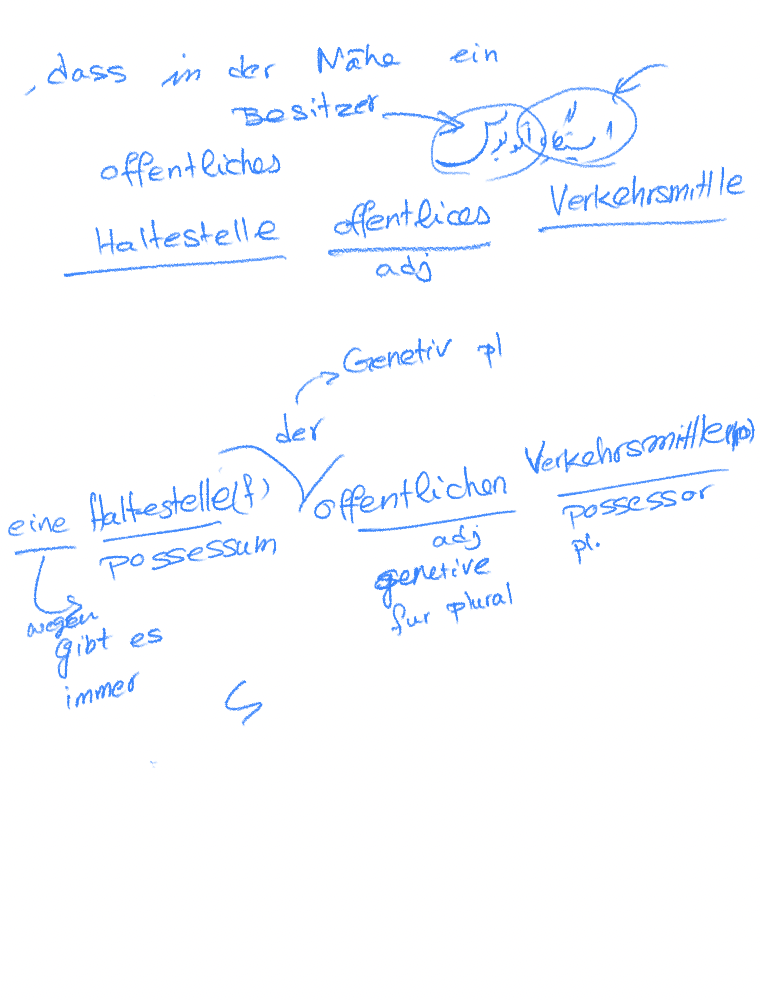
\includegraphics[width=0.9\textwidth]{schreiben_4.png}
               \end{figure}
               Sicherlich, so wie bei(در موردes ist erforderlich im Gegensatz Persisch. immer Dativ) jedem Phänomen(n. ), gibt es(immer mit Akkusativ) auch Nachteile.
               
               \begin{figure}[H]
                  \centering
                  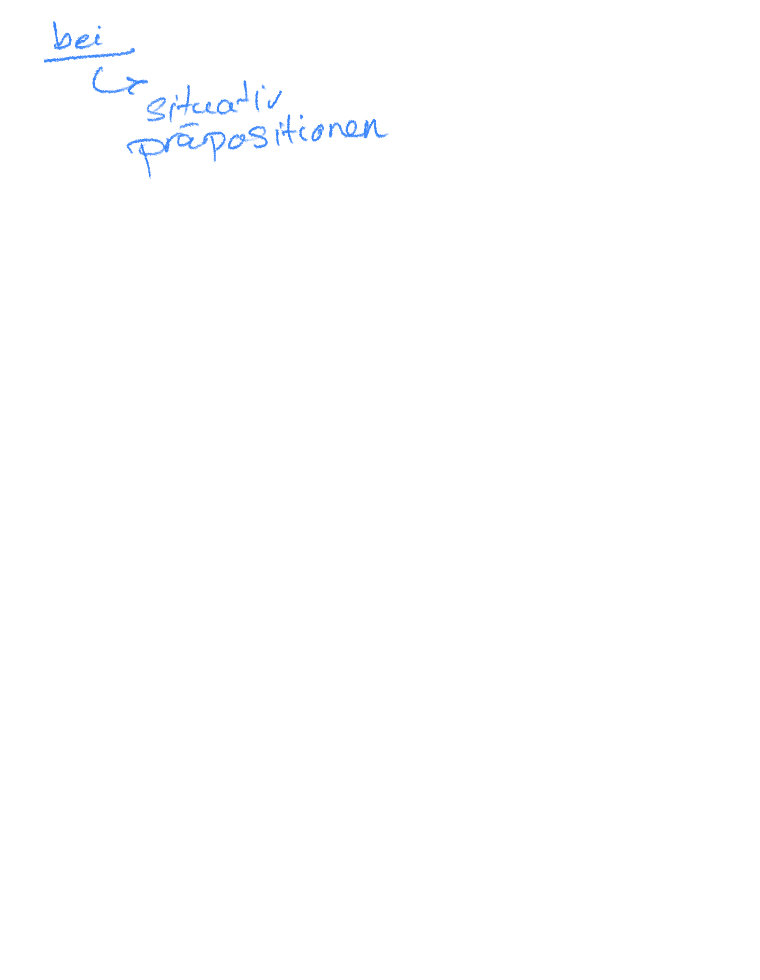
\includegraphics[width=0.9\textwidth]{img_0.png}
               \end{figure}               
   Der erste Nachteil(m.), der in mein Meinung fallen ist, die Wartezeiten, die verloren werden für das nächste Verkehrsmittel um in Haltsstelle zu kommen.  

\end{document}
